\documentclass[tikz,border=10pt]{standalone}
\usepackage{pgfplots}
\pgfplotsset{compat=newest}

\begin{document}

% Q1
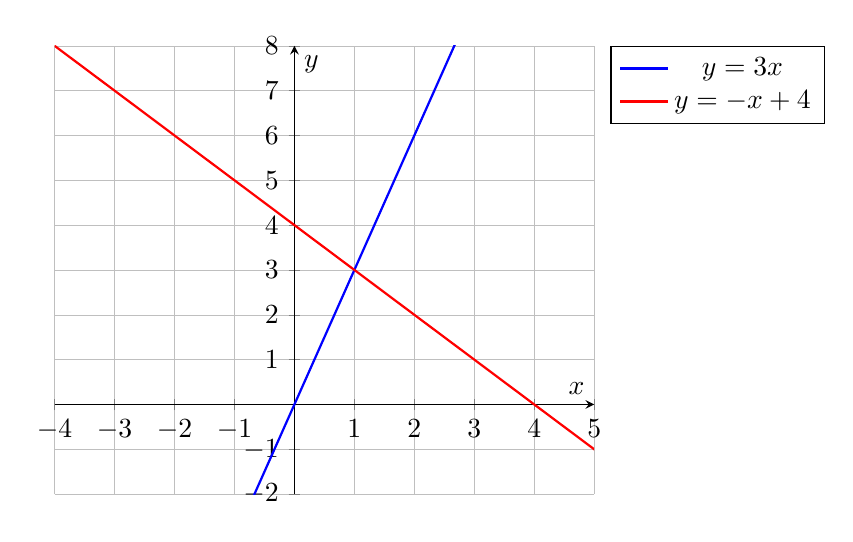
\begin{tikzpicture}
\begin{axis}[
    xlabel={$x$},
    ylabel={$y$},
    axis lines=center,
    grid=both,
    grid style={line width=.1pt, draw=gray!10},
    major grid style={line width=.2pt,draw=gray!50},
    xmin=-4,
    xmax=5,
    ymin=-2,
    ymax=8,
    domain=-10:10,
    smooth,
    no marks,
    xtick={-4,-3,...,5},
    ytick={-2,-1,...,8},
    legend pos=outer north east,
]
\addplot[thick, blue] {3*x};
\addlegendentry{$y = 3x$}
\addplot[thick, red] {-x + 4};
\addlegendentry{$y = -x + 4$}
\end{axis}
\end{tikzpicture}

% Q2
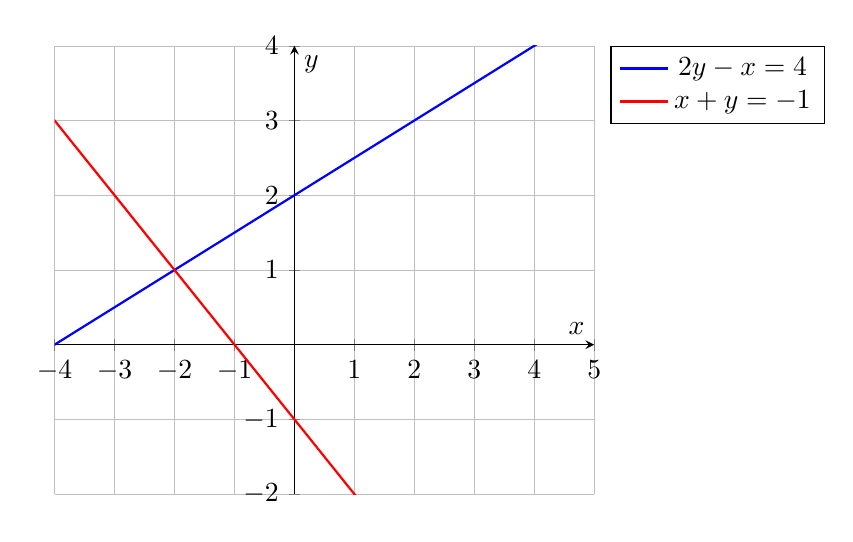
\begin{tikzpicture}
\begin{axis}[
    xlabel={$x$},
    ylabel={$y$},
    axis lines=center,
    grid=both,
    grid style={line width=.1pt, draw=gray!10},
    major grid style={line width=.2pt,draw=gray!50},
    xmin=-4,
    xmax=5,
    ymin=-2,
    ymax=4,
    domain=-10:10,
    smooth,
    no marks,
    xtick={-8,-7,...,5},
    ytick={-4,-3,...,4},
    legend pos=outer north east,
]
\addplot[thick, blue] {x/2 + 2};
\addlegendentry{$2y - x = 4$}
\addplot[thick, red] {-x-1};
\addlegendentry{$x + y = -1$}
\end{axis}
\end{tikzpicture}

% Q3
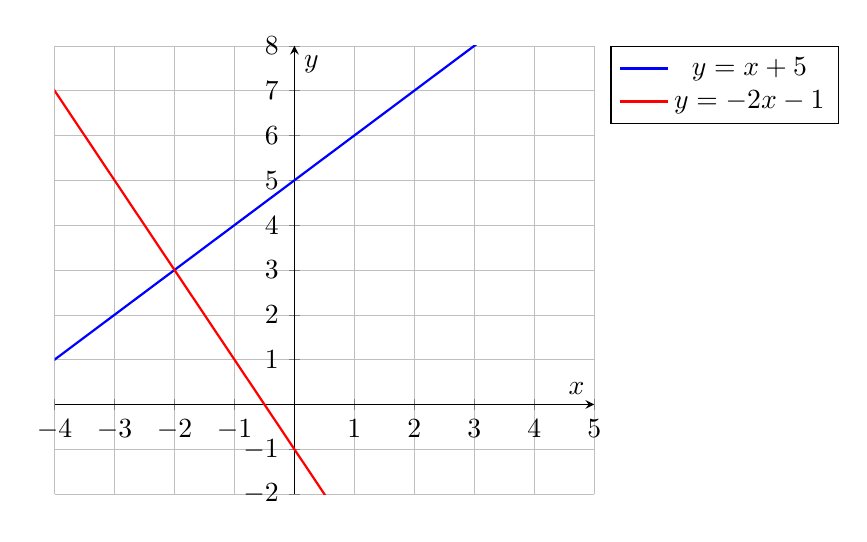
\begin{tikzpicture}
\begin{axis}[
    xlabel={$x$},
    ylabel={$y$},
    axis lines=center,
    grid=both,
    grid style={line width=.1pt, draw=gray!10},
    major grid style={line width=.2pt,draw=gray!50},
    xmin=-4,
    xmax=5,
    ymin=-2,
    ymax=8,
    domain=-10:10,
    smooth,
    no marks,
    xtick={-4,-3,...,5},
    ytick={-2,-1,...,8},
    legend pos=outer north east,
]
\addplot[thick, blue] {x + 5};
\addlegendentry{$y = x + 5$}
\addplot[thick, red] {-2*x - 1};
\addlegendentry{$y = -2x - 1$}
\end{axis}
\end{tikzpicture}

% Q4
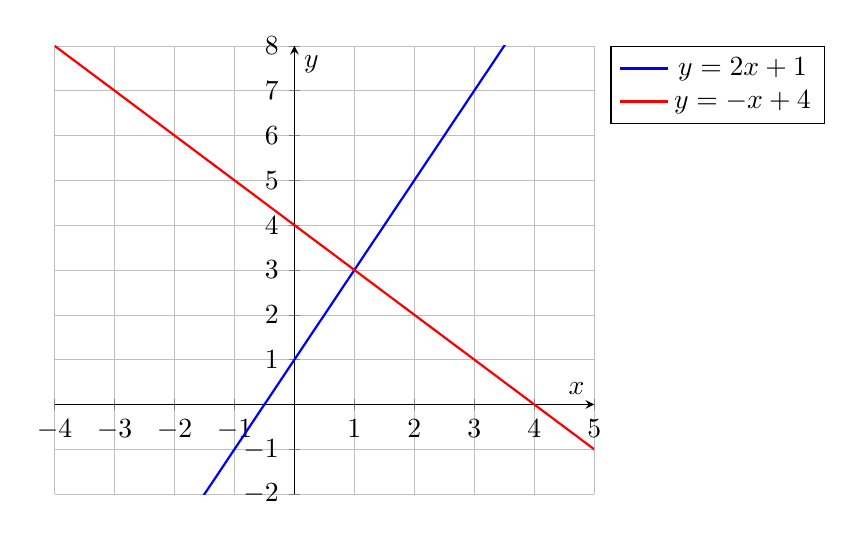
\begin{tikzpicture}
\begin{axis}[
    xlabel={$x$},
    ylabel={$y$},
    axis lines=center,
    grid=both,
    grid style={line width=.1pt, draw=gray!10},
    major grid style={line width=.2pt,draw=gray!50},
    xmin=-4,
    xmax=5,
    ymin=-2,
    ymax=8,
    domain=-10:10,
    smooth,
    no marks,
    xtick={-4,-3,...,5},
    ytick={-2,-1,...,8},
    legend pos=outer north east,
]
\addplot[thick, blue] {2*x + 1};
\addlegendentry{$y = 2x + 1$}
\addplot[thick, red] {-x + 4};
\addlegendentry{$y = -x + 4$}
\end{axis}
\end{tikzpicture}

% Q5
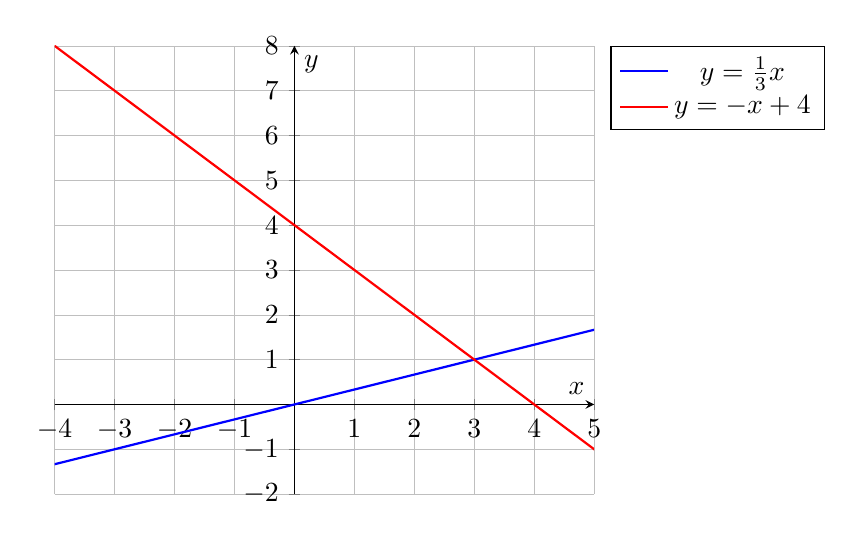
\begin{tikzpicture}
\begin{axis}[
    xlabel={$x$},
    ylabel={$y$},
    axis lines=center,
    grid=both,
    grid style={line width=.1pt, draw=gray!10},
    major grid style={line width=.2pt,draw=gray!50},
    xmin=-4,
    xmax=5,
    ymin=-2,
    ymax=8,
    domain=-10:10,
    smooth,
    no marks,
    xtick={-4,-3,...,5},
    ytick={-2,-1,...,8},
    legend pos=outer north east,
]
\addplot[thick, blue] {(1/3)*x};
\addlegendentry{$y = \frac{1}{3}x$}
\addplot[thick, red] {-x + 4};
\addlegendentry{$y = -x + 4$}
\end{axis}
\end{tikzpicture}

% Q6
\begin{tikzpicture}
\begin{axis}[
    xlabel={$x$},
    ylabel={$y$},
    axis lines=center,
    grid=both,
    grid style={line width=.1pt, draw=gray!10},
    major grid style={line width=.2pt,draw=gray!50},
    xmin=-5,
    xmax=5,
    ymin=-5,
    ymax=5,
    domain=-10:10,
    smooth,
    no marks,
    xtick=\empty,
    ytick=\empty,
    legend pos=outer north east,
]
\addplot[thick, blue] {(2*x+5};
\addlegendentry{$y = 2x+5$}
\addplot[thick, red] {-x -1};
\addlegendentry{$y = -x -1$}
\end{axis}
\end{tikzpicture}

% Q7
\begin{tikzpicture}
\begin{axis}[
    xlabel={$x$},
    ylabel={$y$},
    axis lines=center,
    grid=both,
    grid style={line width=.1pt, draw=gray!10},
    major grid style={line width=.2pt,draw=gray!50},
    xmin=-5,
    xmax=5,
    ymin=-5,
    ymax=5,
    domain=-10:10,
    smooth,
    no marks,
    xtick=\empty,
    ytick=\empty,
    legend pos=outer north east,
]
\addplot[thick, blue] {(-2*x+5};
\addlegendentry{$y = -2x+5$}
\addplot[thick, red] {3*x + 2};
\addlegendentry{$y = 3x +2$}
\end{axis}
\end{tikzpicture}


\end{document}
